\documentclass[11pt,a4paper]{article}
\usepackage[T1]{fontenc}
\usepackage[margin=22mm]{geometry}
\usepackage{graphicx,booktabs,amsmath}
\setlength{\parindent}{0pt}
\setlength{\parskip}{5pt}
\begin{document}
\section*{Reproduction of Rogelio's CSA noise simulation}
The received Spice2 schematic is simulated with its original device dimensions,
biases, 250 fF external input capacitance and 3 fF feedback capacitance.
LTspice 17.2.4 uses the default temperature of 27 degrees Celsius.
A derived model copy replaces NMOS NOIBE with NOIB and closes both model
parameter lists. All numerical coefficients are preserved.
The noise sweep is 1 Hz to 1 GHz, with 1000 points per decade. A second sweep
starts at 0.1 Hz to match the supplied screenshot. All results below use the
extended sweep. The supplied BSIM3 noise parameters are design inputs from
Rogelio; this reproduction does not establish their process calibration.

\begin{center}
\begin{tabular}{rrrr}\toprule
$f$ (Hz) & Total (mV/$\sqrt{\mathrm{Hz}}$) & M1 flicker ($\mu$V/$\sqrt{\mathrm{Hz}}$) & Flicker variance (\%)\\\midrule
0.1 & 20.1667 & 475.708 & 5.428 \\
1 & 3.40497 & 78.876 & 8.801 \\
10 & 0.473628 & 20.7649 & 52.02 \\
100 & 0.122775 & 5.5953 & 92.76 \\
1000 & 0.0412785 & 1.50803 & 98.48 \\
1e+06 & 0.000564871 & 0.00392014 & 16.08 \\
1e+09 & 5.68387e-07 & 6.34864e-08 & 0.02681 \\
\bottomrule\end{tabular}
\end{center}
Flicker contributions are nonzero for all seven transistors. The last column
includes all transistor flicker sources. M1 alone does not represent the
whole circuit. The input-noise trace is equivalent current noise; output
traces are amplitude spectral densities.

At 0.1 Hz, the total output noise is 20.17 mV/$\sqrt{\mathrm{Hz}}$,
and M1 flicker is 475.7 $\mu$V/$\sqrt{\mathrm{Hz}}$.
These scales agree with the supplied screenshot (about 20 mV and 500 $\mu$V,
respectively). The received plot file contains presentation settings rather
than numerical data, so this comparison is limited by the screenshot.

The operating-point change is 0, and the maximum relative gain change is
0. The device variances sum to the output variance with maximum
relative error 6.66e-16. The independently started noise sweeps agree at
common frequencies to 6.33e-14 relative error. Each device's individual
noise mechanisms also sum to its total variance within $10^{-10}$.
The solver reaches the operating point using Gmin stepping. It retains the
original warnings about unspecified diffusion perimeters and the isolated
charge-monitor node; no unknown model parameters are reported.

\begin{center}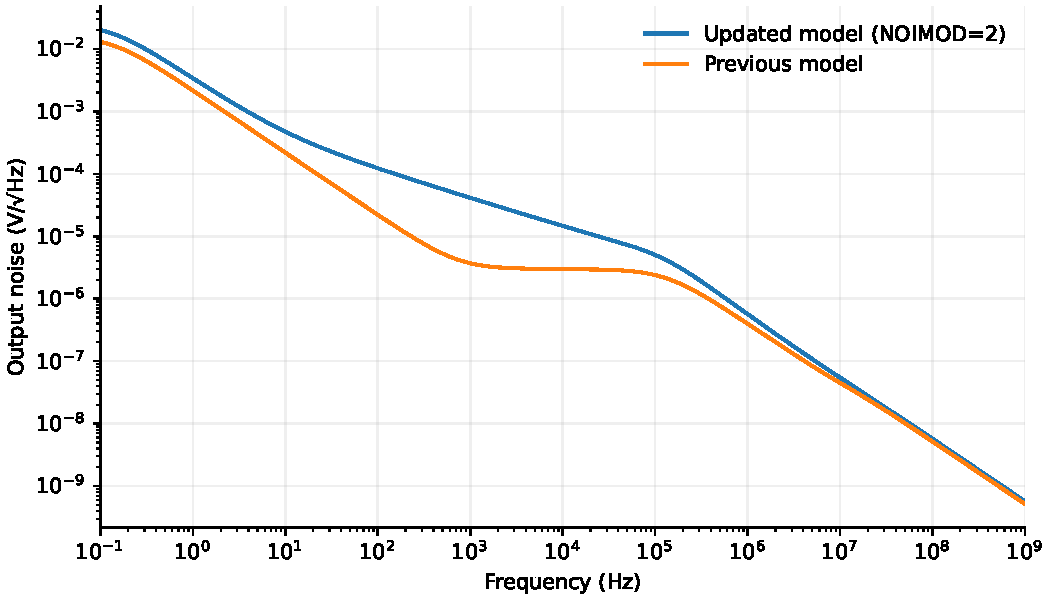
\includegraphics[width=.9\linewidth]{noise_comparison.pdf}\end{center}
\clearpage
\begin{center}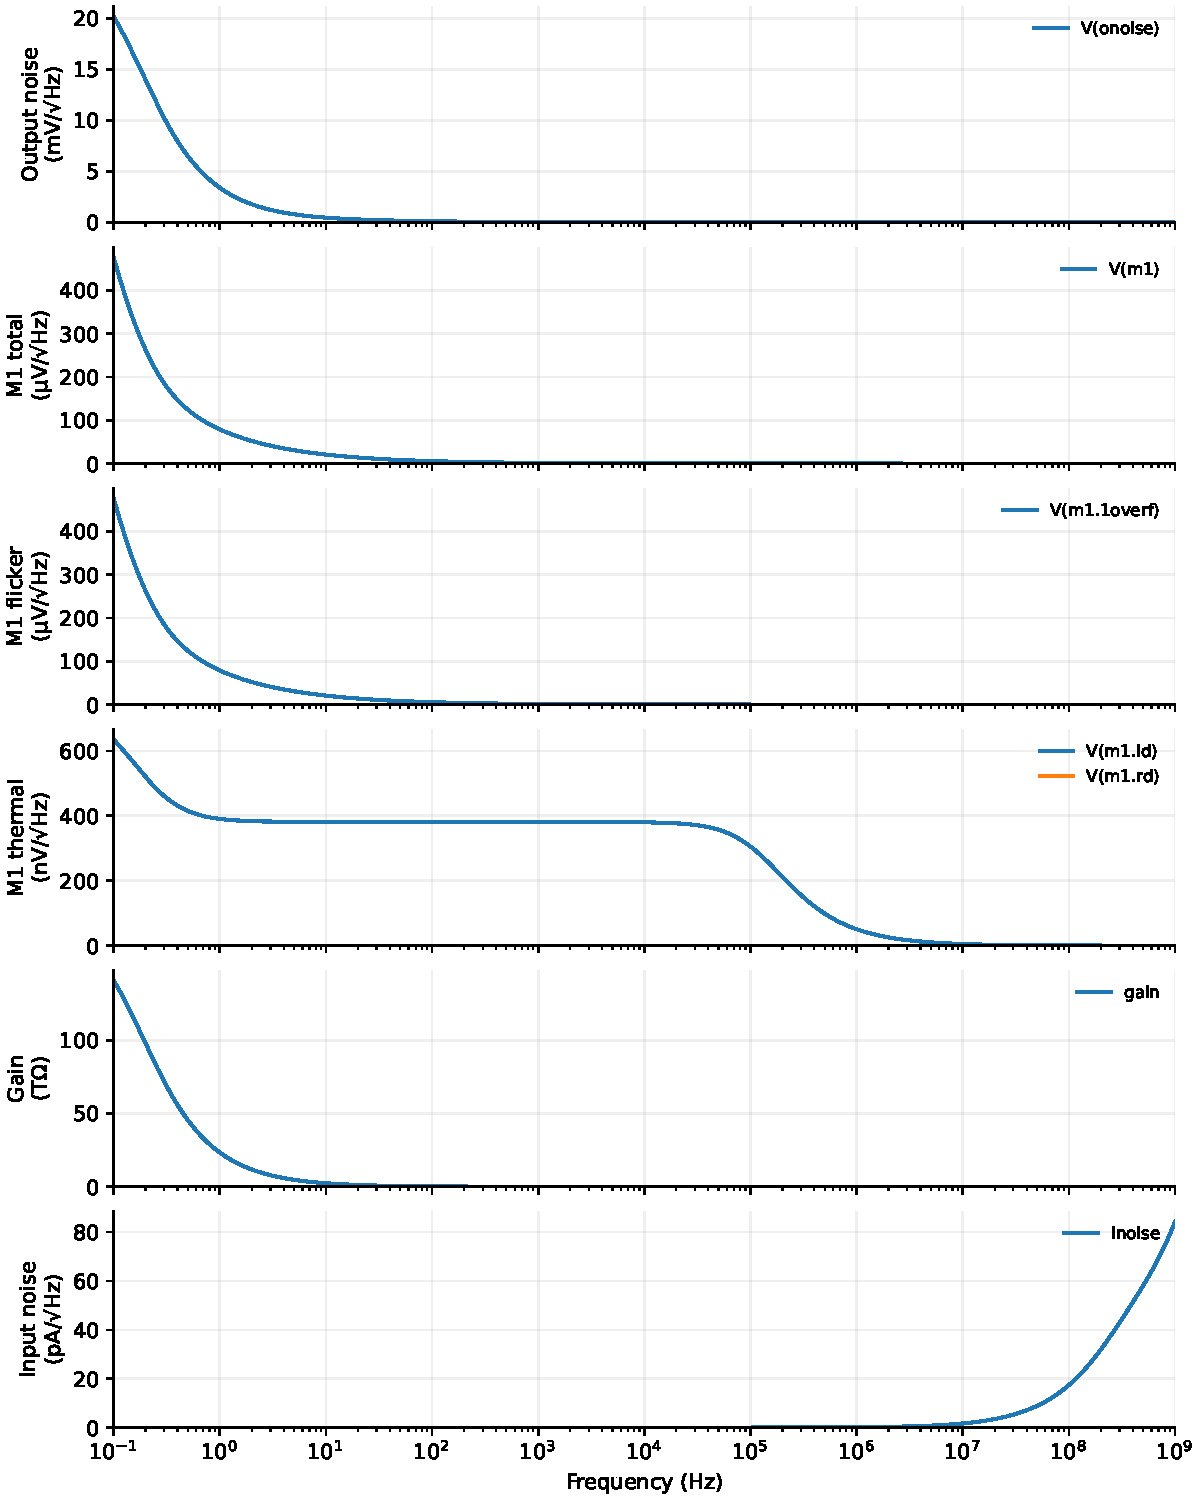
\includegraphics[height=.91\textheight]{noise_reproduction.pdf}\end{center}
\end{document}
